\section{Market Microstructure and Characteristics}

Market microstructure is the study of the mechanics of trading in place 
in real markets. It describes why trading occurs, the rules of trading 
and the protocols to form a trade. \citep[p. 3-4]{Has07}
Understanding market microstructure in designing an artificial market
is vital as without realistic trading settings the artifical market 
has limited practicality. In addition to microstructure, it is important
to understand the general price dynamics in order to validate representativeness
of the artifical market model. In this section, the most common 
properties of real markets and price phenomena are presented. 

% Maybe extend with behavioural aspects?

\subsection{Double Auction}
% Call-market (Itayose, Sealed-bid) vs CDA (Zaraba)

Double auction market is widely used market structure in real 
financial markets. It is a form of auction 
in which both sides of the markets, buyers and sellers, are able to 
produce quotes \citep*{Kle99}. These quotes form the order book 
which is a collection of pending bid and ask offers. A trade 
occurs between crossing and matching orders: each trade is formed between 
a bid order with a higher or equal price and an ask order with a lower 
or equal price \citep*{Ben12}. Double auctions varies in
several aspects: when the orders are matched and how the orders are matched. 
In some implementations, such as \citet*{God93}'s, a trade is 
formed only when a buyer and a seller each agree on the exact trade 
price but typically the matching of crossing orders is automated.

% \subsubsection{Order Matching in Double Auction}

Main distinction between double auction market models is when
the order matching takes place. Typically, the order matching 
is continuous process occuring after the arrival of each new order but
in some markets this process takes place after a specified time interval
has passed, for example at the end of a trading day. \citep{boer05}
In auction literature, there are various terms used to describe essentially 
the same mechanics. \citet{boer05} used term 
\textit{call-market} for the former and \textit{continuous session market}
for the latter whereas \citet{ASt05} called them \textit{Itayose method}
and \textit{Zaraba method} respectively. \citet{Moc15} used term 
\textit{periodic double auction} to describe the same mechanics of call-markets as  which
they described is an extension of a sealed-bid auction. Sealed-bid auctions
is an auction model in which the bid and ask offers
are submitted once and then the order matching is executed once. 

In artificial market literature...
% More about Sealed-bid matching (supply-demand) and CDA matching

\subsection{Execution Systems}
% Quote-driven vs Order-driven
The execution systems are typically divided into two types:
quote-driven and order-driven. In quote-driven market, also known
as intermediate markets, the investors trade with prices provided 
by dealers who are part of the market organization. 
In order-driven market, also called as limit order market, 
the prices are formed according to the orders submitted by the 
investors themselves and trades are formed via automatic order matching 
or market makers. \citep{Baru17}. According to \citet{MALINOVA2013104},
the liquidity and price efficiency are generally better in order-driven 
markets. They also found out that smaller orders get better price in 
quote-driven markets due to smaller bid-ask spread 
but larger orders benefit from order-driven markets because of the lower 
execution costs. Real markets however are most often a combination
of the two \citep{boer05}.

As simulating intermediate market participants increases compexity
of the model, artificial markets with realistic quote-driven execution are rare. 
However, some artificial markets, such as \citet{SantaFe99}'s, do have some of 
the elements of quote-driven markets in a sense that the prices are driven by 
the sizes of the orders and not prices offered by the investors or traders. 
Most of the artificial markets found in the literature seem to be order-driven.


\subsection{Price Formation}
% Order book, matching and clearing
The price formation in a quote-driven market is dependent on how the 
intermediaries or dealers view the supply and demand of the traded
asset thus it is challenging to describe the processes from order submission
to trade formation accurately maintaining a sufficient degree of generalization.
As essentailly the order sizes are only submitted to the market, the market
structure itself bears the responsibility to come up with prices that realistically
represent the fair price of an asset at any given time. Because of these 
factors, quote-driven was not considered for the market structure built in this
thesis and its mechanics is not discussed with more details.

On the otherhand, all order-driven markets share the same abstraction regarding
to price formation. The submitted orders in order driven market form the limit order 
book which is the key element for these markets. Limit order is an order that
consists of quantity and price, and often also the issued timestamp.
There of course exists other types of orders than limit orders but these can be seen as derivatives from limit
orders: for example, a bid (an ask) market order is essentially a limit order 
with an extremely high (low) price so that it does get matched regardless of the
state of the order book. \citep{lob13} A simple order book is visualized in ~\ref{fig:lob_repr}
with relevant terminology.

\begin{figure}
    \begin{center}  
        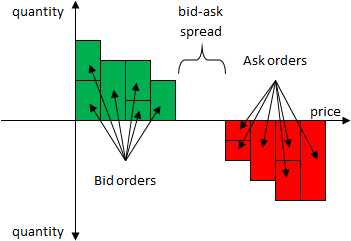
\includegraphics[width=7.5cm]{diagrams/lob_repr.png}
        \caption{Simple representation of a limit order book}
        \label{fig:lob_repr}
    \end{center}
\end{figure}

\citet{lob13} explained thorougly the price mechanics in continuous market. I 
further generalize their explanation to include also periodical auctions.
When clearing occurs, bid orders are matched with ask orders in a way that a 
trade forms between a bid with a price p\textsubscript{b} and an ask with a price 
p\textsubscript{a} where p\textsubscript{b} $\geq$ p\textsubscript{a}. However, it is likely
that not all the bids that have higher price than the lowest ask and not all the asks that
have lower price than the highest bid in the market can be matched due to the asymmetricity 
of quantity per price level. A simple illustration of the order book evolution is presented
in the figure ~\ref{fig:lob_evo}: the order book receives two new bids in t, bids 1 and 2.
On t + 1, clearing occurs and the bid 2 is matched with one of the equal sized best ask orders.
Bid 1 is left in the order book and becomes the best bid order. As the order prices differ
between the bid 2 and the corresponding ask, it is not entirely obvious which price to pick
for the trade: bid's price, ask's price or the average. Especially in continuous markets,
the trade price is set according to the order that was in the order book already, in this
example the ask order. % Something about supply demand price matching etc.

\begin{figure}
    \begin{center}  
        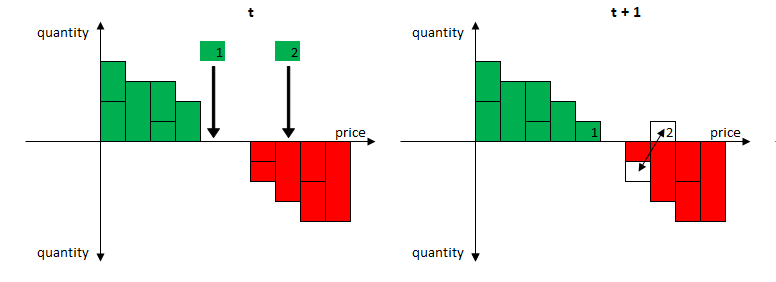
\includegraphics[width=15cm]{diagrams/lob_evolution.png}
        \caption{Evolution of a limit order book}
        \label{fig:lob_evo}
    \end{center}
\end{figure}

\subsection{Price Dynamics}
% Stylized facts
The price dynamics in stock markets are known to be chaotic and difficult to 
analyze. The underlying elements that play a role in the price formation
are constantly evolving and it still remains relatively poorly understood.
However, there are some characteristics of price behaviour that are supported
with enough empirical evidence to be considered as properties of price in
financial markets. These statistical phenomena, called stylized facts in
econometrics, have been observed in extensive amount of studies from 
different assets, markets and time periods \citep{Shakeel18}. 
% List of Stylized facts (Cont R. (2001) & Gould et al. (2013))
The price related stylized facts are according to \citet{StylizedFacts01} and \citet{lob13}:

\begin{enumerate}
    \item Fat-tailed distribution of returns: distribution of asset returns have fatter tails than normal distribution. Returns have positive excess kurtosis. 
    \par
    \begin{minipage}{\linewidth}
        \centering
        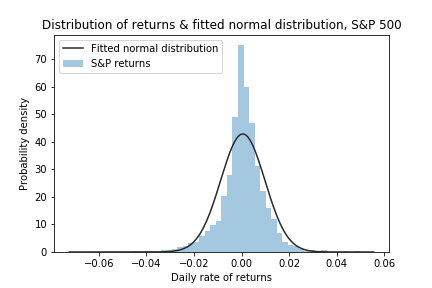
\includegraphics[width=10cm]{plots/S&P500_fat_tails.png}
        \captionof{figure}{Example of fat-tailed of returns}
    \end{minipage}

    \item Lack of autocorrelation: autocorrelation of returns in financial markets have shown to be statistically insignificant except in very short term. Previous return has no prediction power over the following. 
    \par
    \begin{minipage}{\linewidth}
        \centering
        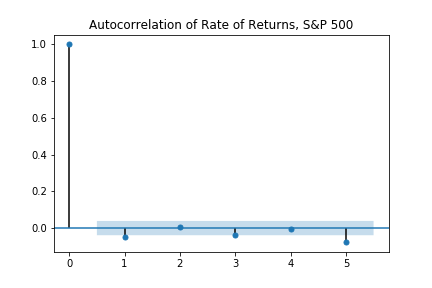
\includegraphics[width=10cm]{plots/S&P500_autocorr.png}
        \captionof{figure}{Example of absense of autocorrelation}
    \end{minipage}

    \item Volatility clusters: volatility have measured to have positive autocorrelation. Strong price movement tend to follow additional exceptional price movements forming clusters of volatility in time.
    \par
    \begin{minipage}{\linewidth}
        \centering
        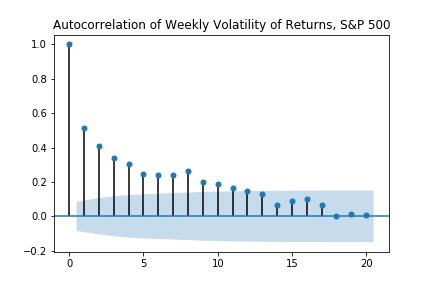
\includegraphics[width=10cm]{plots/S&P500_vola_autocorr.png}
        \captionof{figure}{Example of volatility clustering}
    \end{minipage}
\end{enumerate} 

% Something about theories of these things (explanation for the stylized facts)
% file:///D:/Opinnot/Master's%20Thesis/literature/real%20markets/price%20dynamics/TheoriesExplainingStockPriceBehavior%20(1).pdf

As has been done in the previous literature of artificial markets, the 
representativeness of the ASM built in this thesis is validated also 
using these stylized facts.